\documentclass{article}
% 导入导言区
% 该文件仅负责格式配置或通用命令
% 只适用于该论文的自定义命令放到 预定义.tex
% 中文
\usepackage{ctex}
% 浮动体控制
\usepackage{float}
% 长表格
\usepackage{longtable}
% 页面大小
\usepackage[left=2.5cm,right=2cm,top=2.5cm,bottom=2cm]{geometry}
% 解决字体警告
\usepackage{anyfontsize}
% 设置英文字体
\setmainfont{Times New Roman}
% 图片宏包
\usepackage{graphicx}
% 图片文件夹路径
\graphicspath{{../Output/}}
% 摘要强调
\newcommand{\absemph}[1]{\textbf{#1}}
% 规定论文格式
\usepackage{gbt7714}
% 颜色
\usepackage{xcolor}
% 字体
\usepackage{fontspec}
% 间距控制
\usepackage{setspace}
% 子图
\usepackage{subfigure}
% 页眉页脚
\usepackage{fancyhdr}
\pagestyle{fancy}
\fancyhf{}
\fancyhead[C]{\songti\zihao{5}河北农业大学学士学位论文}
\fancyfoot[C]{\zihao{5}\thepage}
% 章节格式
\usepackage{titlesec}
% 设置章节格式
\titleformat{\section}{\centering\heiti\zihao{-3}}{第\arabic{section}章}{1em}{}
\titleformat*{\subsection}{\heiti\zihao{4}}
\titleformat*{\subsubsection}{\heiti\zihao{-4}}
% 数学相关宏包
\usepackage{amsmath,amssymb,mathrsfs}
% 图表公式章节编号
\renewcommand{\thetable}{\thesection-\arabic{table}}
\renewcommand{\thefigure}{\thesection-\arabic{figure}}
\renewcommand{\theequation}{\thesection.\arabic{equation}}
\makeatletter
\@addtoreset{table}{section}
\@addtoreset{figure}{section}
\@addtoreset{equation}{section}
\makeatother
% 超链接
\usepackage[
      colorlinks,
      linkcolor=black,
      anchorcolor=black,
      citecolor=black
]{hyperref}
% 流程图
\usepackage{tikz}
\usetikzlibrary{shapes.geometric,arrows}
\tikzstyle{startstop} = [rectangle,rounded corners, minimum width=1cm,minimum height=1cm,text centered, draw=black,fill=red!30]
\tikzstyle{io} = [trapezium, trapezium left angle = 70,trapezium right angle=110,minimum width=1cm,minimum height=1cm,text centered,draw=black,fill=blue!30]
\tikzstyle{process} = [rectangle,minimum width=1cm,minimum height=1cm,text centered,text width =1cm,draw=black,fill=orange!30]
\tikzstyle{decision} = [diamond,minimum width=1cm,minimum height=1cm,text centered,draw=black,fill=green!30]
\tikzstyle{arrow} = [thick,->,>=stealth]
% 英文摘要
\newenvironment{enabstract}{
      \par\small
      \noindent\mbox{}\hfill{\bfseries \zihao{-3} ABSTRACT}\hfill\mbox{}\par
      \vskip 2.5ex}{\par\vskip 2.5ex}
% 中文摘要
\newenvironment{cnabstract}{
      \par\small
      \noindent\mbox{}\hfill{\bfseries \heiti\zihao{-3} 摘  要}\hfill\mbox{}\par
      \vskip 2.5ex}{\par\vskip 2.5ex}
% 代码环境
\usepackage{listings}
% 代码格式设置
\lstset{
      % 语言
      language=python,
      % 自动换行
      breaklines=true,
      % 行号
      numbers=left,
      % 字符串显示空格
      showstringspaces=false,
      % 基础字体设置
      basicstyle=\small\fontspec{Monaco},
      % 字符串风格
      stringstyle=\color{purple},
      % 注释风格
      commentstyle=\color{gray},
      % 关键字风格
      keywordstyle=\color{blue},
      % 左侧margin
      xleftmargin = 25pt,
      % 添加frame
      frame = tb,
      % 设置frame左侧margin
      framexleftmargin = 20pt,
}
% 导入预定义指令
% SIR模型
\def\SIR{
    \begin{table}[H]
        \centering
        \caption{SIR模型参数表}
        \begin{tabular}{ll}
            \hline
            符号     & 含义         \\
            \hline
            $\alpha$ & \PText{S}{I} \\
            $\beta$  & \PText{I}{R} \\
            \hline
        \end{tabular}
    \end{table}
    \def\SI{IS\alpha}
    \def\IR{I\beta}
    \begin{align}
        \dt{S} & = -\SI      \\
        \dt{I} & = \SI - \IR \\
        \dt{R} & = \IR
    \end{align}
}
\def\SEIR{
    \begin{table}[H]
        \centering
        \caption{SEIR模型参数表}
        \begin{tabular}{ll}
            \hline
            符号       & 含义         \\
            \hline
            $\alpha$   & \PText{S}{E} \\
            $\gamma$   & \PText{E}{I} \\
            $\epsilon$ & \PText{E}{R} \\
            $\beta$    & \PText{I}{R} \\
            \hline
        \end{tabular}
    \end{table}
    \def\SE{(I+E)S\alpha}
    \def\EI{E\gamma}
    \def\ER{E\epsilon}
    \def\IR{I\beta}
    \begin{align}
        \dt{S} & = -\SE            \\
        \dt{E} & = \SE - \EI - \ER \\
        \dt{I} & = \EI - \IR       \\
        \dt{R} & = \IR +\ER
    \end{align}
}
\def\SEIRD{
    \begin{table}[H]
        \centering
        \caption{SEIRD模型参数表}
        \begin{tabular}{ll}
            \hline
            符号       & 含义         \\
            \hline
            $\alpha$   & \PText{S}{E} \\
            $\gamma$   & \PText{E}{I} \\
            $\epsilon$ & \PText{E}{R} \\
            $\beta$    & \PText{I}{R} \\
            $\delta$   & \PText{I}{D} \\
            \hline
        \end{tabular}
    \end{table}
    \def\SE{(I+E)S\alpha}
    \def\EI{E\gamma}
    \def\ER{E\epsilon}
    \def\IR{I\beta}
    \def\ID{I\delta}
    \begin{align}
        \dt{S} & = -\SE            \\
        \dt{E} & = \SE - \EI - \ER \\
        \dt{I} & = \EI - \IR - \ID \\
        \dt{R} & = \IR + \ER       \\
        \dt{D} & = \ID
    \end{align}
}
\def\SEIRS{
    \begin{table}[H]
        \centering
        \caption{SEIRS模型参数表}
        \begin{tabular}{ll}
            \hline
            符号       & 含义         \\
            \hline
            $\alpha$   & \PText{S}{E} \\
            $\gamma$   & \PText{E}{I} \\
            $\epsilon$ & \PText{E}{R} \\
            $\beta$    & \PText{I}{R} \\
            $\delta$   & \PText{I}{D} \\
            $\theta$   & \PText{R}{I} \\
            \hline
        \end{tabular}
    \end{table}
    \def\SE{(I+E)S\alpha}
    \def\EI{E\gamma}
    \def\ER{E\epsilon}
    \def\IR{I\beta}
    \def\ID{I\delta}
    \def\RI{R\theta}
    \begin{align}
        \dt{S} & = -\SE                  \\
        \dt{E} & = \SE - \EI - \ER       \\
        \dt{I} & = \RI + \EI - \IR - \ID \\
        \dt{R} & = \IR - \RI + \ER       \\
        \dt{D} & = \ID                   \\
    \end{align}
}
\title{\heiti \zihao{-2} 基于SEIR的病毒传播模型}
\author{\songti \zihao{-4} 信息与计算科学 1601 骆天奇\\指导教师\ 王斌}
\date{}
\begin{document}
\begin{titlepage}
      \thispagestyle{empty}
      \begin{center}
      \vspace{2cm}
      \includegraphics[height=3cm]{logo_pic.jpg}\hspace{0.3cm}
      \includegraphics[height=3cm]{logo_name.jpg}\\
      \vspace{1cm}
      \text{\heiti\zihao{0}学士学位论文}
      \vspace{2cm}
      \begin{spacing}{2.0}
            \text{\heiti\zihao{1}基于SEIR的病毒传播模型}
      \end{spacing}
      \vspace{4cm}
      \zihao{3}
      \songti
      \begin{tabular}[b]{cl}
            \rule{0pt}{1cm}\text{姓  名} & 骆天奇             \\%\cline{2-2}
            \rule{0pt}{1cm}\text{学  号} & 2016254060407      \\%\cline{2-2}
            \rule{0pt}{1cm}\text{院  系} & 理学院             \\%\cline{2-2}
            \rule{0pt}{1cm}\text{专  业} & 信息与计算科学1601 \\%\cline{2-2}
            \rule{0pt}{1cm}\text{指导教师} & 王斌               \\%\cline{2-2}
      \end{tabular}
      \\
      \vspace{3cm}
      \textbf{二〇二〇 年 五 月 二十 日}
\end{center}
\clearpage
      \thispagestyle{empty}
      \vspace{2cm}
\begin{center}
    \textbf{\zihao{3}论文原创性声明内容}
\end{center}
\par 本人郑重声明:
所呈交的学位论文《基于SEIR的病毒传播模型》,
是本人在导师的指导下,
独立进行研究工作所取得的成功。
除文中已经注明引用的内容外,
本论文不包含任何其他个人或集体已经发表或撰写过的作品成果。
对本文的研究做出重要贡献的个人和集体,
均已在文中以明确方式标明。
本人完全意识到本声明的法律结果由本人承担。
\vspace{2cm}\\
\begin{table}[H]
    \begin{tabular}{l}
        \vspace{1cm}
        学位论文作者签名:\hspace{6cm} \\
        \vspace{1cm}
        \hspace{2cm}年\hspace{1cm}月\hspace{1cm}日
    \end{tabular}
\end{table}
\vspace{4cm}
\begin{center}
    \textbf{\zihao{3}学位论文使用授权声明}
\end{center}
\par 本人完全了解河北农业大学有关保留、使用学术论文的规定,
即:学校有权保留学位论文并向国家主管部门或指定机构送交论文的电子版和纸质版,
有权将学位论文用于非盈利目的的少量复制并允许论文进入学习图书馆、院系资料室被查阅,
有权将学位论文的内容编入有关数据库进行检索,
可以采用复印、缩印或其他方法保存学位论文。
\vspace{2cm}
\begin{table}[H]
    \begin{tabular}{ll}
        \vspace{1cm}
        学位论文作者签名:\hspace{6cm}             & 导师签名: \\
        \vspace{1cm}
        \hspace{2cm}年\hspace{1cm}月\hspace{1cm}日 &
        \hspace{2cm}年\hspace{1cm}月\hspace{1cm}日
    \end{tabular}
\end{table}
\clearpage
      % 大写罗马页码
      \pagenumbering{Roman}
      \setcounter{page}{1}
      \maketitle
      % 摘要
\begin{cnabstract}
    \songti \zihao{-4}
    \absemph{目的:}
    在$SEIR$模型的基础上结合COVID-19病毒的特点创建衍生模型,
    在所建立的模型中找出一个与该疫情拟合度最高的病毒传播模型。
    使用最优模型对该病毒传播进行分析。
    \absemph{方法:}
    基于$SEIR$病毒传播模型,
    根据病毒特点构建新的衍生模型。
    并使用官方公布的数据进行拟合,
    根据拟合效果选择最优模型。
    \absemph{结果:}
    在本文提到的几个模型中,
    通过对比模型与实际数据的拟合程度优劣,
    判断加入死亡人群$D$的$SEIR$模型最符合疫情传播趋势,
    并通过分析最优模型的最优估计参数来计算病毒的基本生殖数$R_0$和有效生殖数$R_t$。
    计算出整个疫情期间的$R_t=1.754$,
    并通过数据分段拟合计算出疫情的初期$R_0=5.937$,
    以及疫情后期$R_t=1.081$。
    所得结论与官方数据及文献相符,
    说明该模型可以较为准确的描述疫情传播过程。
    \\
    \absemph{关键字:} SEIR, 数学模型,传染病, COVID-19
\end{cnabstract}
\begin{enabstract}
    \zihao{-4}
    \absemph{Target:}
    Based on the $ SEIR $ model,
    combined with the characteristics of the COVID-19 virus to create a derivative model,
    find a virus propagation model with the best fit to the epidemic in the established model.
    Use the optimal model to analyze the spread of the virus.
    \absemph{Method:}
    Based on the $ SEIR $ virus propagation model,
    a new derivative model is constructed according to the characteristics of the virus.
    And use the officially published data for fitting,
    and select the optimal model according to the fitting effect.
    \absemph{Result:}
    Among the several models mentioned in this article,
    by comparing the fit of the model with the actual data,
    it is judged that the $ SEIR $ model that joins the death crowd $ D $ is most in line with the epidemic transmission trend,
    and by analyzing the optimal model Estimate the parameters to calculate the basic reproduction number of the virus $ R_0 $ and the effective reproduction number $ R_t $.
    Calculate the $ R_t = 1.754 $ for the entire epidemic period,
    and calculate the initial $ R_0 = 5.937 $ of the epidemic and the later $ R_t = 1.081 $ of the epidemic by fitting the data piecewise.
    The conclusions obtained are consistent with official data and literature,
    indicating that the model can describe the epidemic transmission process more accurately.
    \\
    \absemph{Key Words:} SEIR, mathematical model, epidemic, COVID-19
\end{enabstract}
      \clearpage
      \tableofcontents
\end{titlepage}
% 数字页码
\pagenumbering{arabic}
\songti \zihao{-4}
\section{引言}
\subsection{研究背景}
新型冠状病毒疫情发生以来,
引起全世界众多政府、民众、媒体的关注,
并有众多专家学者针对疫情做出一系列研究成果。
国内各部门和地方组织在
疫情防控、患者救治、科研攻关、物资保障
等方面采取了一系列措施。
传染病的扩散对人们的健康和生命安全造成了巨大威胁,
同时严重影响了社会生活和国民经济。
了解疫情的传播情况可以提前做好医疗资源的配备,
有序进行复工复产的安排并坚定人们战胜疫情的信心,
因此构建一个该类病毒的传播模型是有价值的。
\subsection{研究目的}
新型冠状病毒(COVID-19)的爆发引起了国内外众多关注,
预测传染病的传布趋势可以大致得知疫情蔓延趋势及结束时间以提前做出安排。
本文希望通过构建$SEIR$模型及其多个衍生模型,
结合COVID-19的疫情数据进行拟合分析,
探究传染病的传播规律并预测其发展趋势。
在尝试的几种模型中找寻适合用于此类病毒的模型。
\section{研究基础}
\subsection{研究概况}
疫情发生以来,
众多国内外不同领域的专家学者对此高度关注,
从各个层面深度剖析,
运用各种方法预测疫情趋势。
其中以基于$SIR$模型的$SEIR$模型最为多见,
众多专家学者依据COVID-19的特点通过$SEIR$模型进行拟合分析,
得出诸多研究成果。
\subsection{文献综述}
\input{文献综述.tex}
\subsection{理论基础}
\par 在介绍$SEIR$模型前,
需要先说明$SIR$模型,
$SEIR$模型是由$SIR$模型发展而来的。
\par \citeauthor{对流行病数学理论的贡献}在\citeyear{对流行病数学理论的贡献}年研究黑死病时提出了仓室模型,模型中将人口分为三类:
\begin{itemize}
    \item 易感者(susceptibles),$S$人群
    \item 感染者(infectives),$I$人群
    \item 康复者(recovered),$R$人群
\end{itemize}
\par 将其称为$SIR$
\cite{对流行病数学理论的贡献}模型。
\citeauthor{Kermack-McKendrick确定性流行病模型的推广}在\citeyear{Kermack-McKendrick确定性流行病模型的推广}年对其进行了推广\cite{Kermack-McKendrick确定性流行病模型的推广},证明其广泛的适用性。
\par $SIR$模型的建立基于几个假设\cite{对流行病数学理论的贡献}:
\begin{itemize}
    \item 人口总数保持常量(包含预测死亡)
    \item 单位时间$t$传染人数与$S$和$I$人数成正比,即$S\to I = \alpha SI$
    \item 单位时间$t$康复人数与$I$成正比,即$I\to R = \beta I$
\end{itemize}
\begin{table}[H]
    \centering
    \caption{SIR模型符号表}
    \label{table:SIR模型符号表}
    \begin{tabular}{ll}
        \hline
        符号     & 含义         \\
        \hline
        S        & 易感者       \\
        I        & 感染者       \\
        R        & 康复者       \\
        $\alpha$ & \PText{S}{I} \\
        $\beta$  & \PText{I}{R} \\
        \hline
    \end{tabular}
\end{table}
\par 感染机制如下:
\begin{align}
    S(t) & \xrightarrow \alpha I(t) \\
    I(t) & \xrightarrow \beta R(t)
\end{align}
\par 可以用积分方程表示为
\begin{align}
    \dt{S} & = -\alpha SI          \label{math:SIR_S}  \\
    \dt{I} & = \alpha SI - \beta I  \label{math:SIR_I} \\
    \dt{R} & = \beta I\label{math:SIR_R}
\end{align}
\par 对式(\ref{math:SIR_S})的说明:
\par 易感者转变为感染者的人数为$\text{易感者}\times\text{接触率}\times\text{感染率}$,
其中接触率为$\frac{\text{感染者}}{\text{总人数}}$。
\par 总人数是一个常数,
规定$\alpha=\frac{\text{感染率}}{\text{总人数}}$,
得出$\dt{S}$:
\begin{align*}
    \dt{S} & = -\text{易感者}\times\text{接触率}\times\text{感染率} \\
           & = -S\cdot\frac{I}{\text{总人数}}\cdot\text{感染率}     \\
           & = -S\cdot I\cdot\frac{\text{感染率}}{\text{总人数}}    \\
           & = -S\cdot I \cdot \alpha
\end{align*}
\par 对式(\ref{math:SIR_R})的说明:
\begin{align*}
    \dt{R} & = \text{感染者}\times\text{治愈率} \\
           & =I\cdot \beta
\end{align*}
\par 对式(\ref{math:SIR_I})的说明:
\begin{align*}
    \dt{I} & = -\dt{S} - \dt{R}                     \\
           & = S\cdot I \cdot \alpha - I\cdot \beta
\end{align*}
\par $SEIR$模型是在$SIR$模型基础上加入病毒携带者$E$(Exposed)得来的,
详细模型将在\ref{sec:SEIR}进行说明。
\subsection{使用工具}
本文使用python实现爬虫动态获取所需数据、
使用scipy库进行高效率的积分求解及数据拟合、
使用pyecharts库绘制较为美观的图像。
\section{模型研究}
\subsection{模型解释}
\par 通过微分方程来描述美观简练,
但在扩建模型时会有一些麻烦:
由表\ref{table:SIR模型符号表}可预见,
随着划分人群的增多,
人群间感染机制也随之复杂,
不同人群之间转变率的符号也会增多或者改变含义,
这会使读者对符号的理解产生负面的路径依赖影响,
对于模型的扩建是十分不利的。
\par $SIR$模型的本质为人群间的转移,
只要理解人群间的转移方程便可了解模型的结构。
而这类模型都是在总人数固定的前提下进行的,
所以通过状态转移方程即可得出微分方程,
传染病问题中,
状态转移等价于感染机制,
为了更为清晰的描述人群间的感染机制,
本文将引入新的描述方式。
\begin{table}[H]
    \centering
    \caption{另一种模型符号表示}
    \begin{tabular}{ll}
        \hline
        符号       & 含义                              \\
        \hline
        $\P{a}{b}$ & a群体变为b群体的概率              \\
        $\T{a}{b}$ & 单位时间$t$内a群体变为b群体的人数 \\
        \hline
    \end{tabular}
\end{table}
\par 将a到b群体的转换概率用$\P{a}{b}$表示,单位时间内a到b群体转变的人数为$\T{a}{b}$。
\par 感染机制如下:
\begin{align}
    S(t)\xrightarrow{\P{S}{I}}I(t) \Rightarrow \TP{S}{I}{SI} \\
    I(t)\xrightarrow{\P{I}{R}}R(t) \Rightarrow \TP{I}{R}{I}
\end{align}
\par 可将其简化为:
\begin{align}
    \TP{S}{I}{SI} \\
    \TP{I}{R}{I}
\end{align}
\par 流程图为:
\begin{figure}[H]
    \centering
    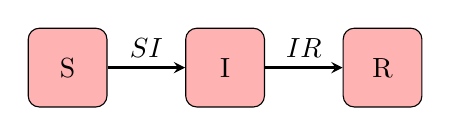
\begin{tikzpicture}[node distance=2cm]
        \node[startstop](S){S};
        \node[startstop,right of=S](I){I};
        \node[startstop,right of=I](R){R};
        \draw[arrow](S)--node[above]{$\T{S}{I}$}(I);
        \draw[arrow](I)--node[above]{$\T{I}{R}$}(R);
    \end{tikzpicture}
    \caption{$SIR$模型流程图}
\end{figure}
\par 易感者转变为感染者,感染者转变为治愈者(包含死亡者)。
\par 将所有人群放到一个集合$\mathbb{A}$中,则模型的积分方程为:
\begin{equation}
    \dt{a} = \sum\left(\T{b}{a}-\T{a}{b}\right)
\end{equation}
\par 其中$a\in\mathbb{A}$,$b\in\mathbb{A}$且$b\not=a$,不在感染机制中的$\T{a}{b}$为$0$。
\par 该积分式对本文中提到的所有模型都适用,
读者通过了解新模型的感染机制$\T{a}{b}$即可了解该模型的结构,
进而宏观的理解整个模型的运作方式。
本文会在介绍模型时首先列出感染机制,
随后给出参数表及详细积分式供读者参考。
\subsection{模型推论}
\par 本文共引入$5$种人群,在此声明。
\begin{table}[H]
    \centering
    \caption{人群}
    \begin{tabular}{ll}
        \hline
        符号 & 含义   \\
        \hline
        $S$  & 易感者 \\
        $I$  & 感染者 \\
        $R$  & 康复者 \\
        $E$  & 携带者 \\
        $D$  & 病逝者 \\
        \hline
    \end{tabular}
\end{table}
\subsubsection{$SEIR$模型}
\par 考虑到易感人群接触到感染者后不会立即患病,
而是经过一段时间潜伏期,
即携带病毒还未患病,
将该类人群定义为携带者人群$E$,
该人群有可能转变为治愈者$R$或感染者$I$,
即为$SEIR$模型。
在COVID-19中这类人群一般会通过检测试剂等方式被诊断为疑似病例。
\paragraph{感染机制}
\begin{align}
    \TP{S}{E}{S(I+E)} \\
    \TP{E}{R}{E}      \\
    \TP{E}{I}{E}      \\
    \TP{I}{R}{I}
\end{align}
\par 流程图为:
\begin{figure}[H]
    \centering
    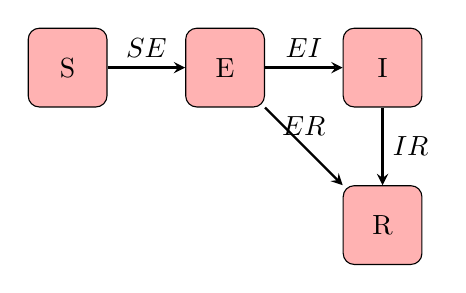
\begin{tikzpicture}[node distance=2cm]
        \node[startstop](S){S};
        \node[startstop,right of=S](E){E};
        \node[startstop,right of=E](I){I};
        \node[startstop,below of=I](R){R};
        \draw[arrow](S)--node[above]{$\T{S}{E}$}(E);
        \draw[arrow](E)--node[above]{$\T{E}{I}$}(I);
        \draw[arrow](E)--node[above]{$\T{E}{R}$}(R);
        \draw[arrow](I)--node[right]{$\T{I}{R}$}(R);
    \end{tikzpicture}
    \caption{$SEIR$模型流程图}
\end{figure}
\par 易感者会转变为携带者,
由于接触携带者也会感染,
故此时接触者为$I+E$,
$\dt{S}$公式变为$-(I+E)S\alpha$,
携带者会转变为治愈者或感染者。
\paragraph{详细积分式}
\SEIR
\subsubsection{$SEIRD$模型}
\par 在$SEIR$的基础上加入死亡人群$D$,
即为$SEIRD$模型。
\par $SEIRD$模型理论上能比$SEIR$模型更精确的描述人群转移状况。
\paragraph{感染机制}
\begin{align}
    \TP{S}{E}{S(I+E)} \\
    \TP{E}{R}{E}      \\
    \TP{E}{I}{E}      \\
    \TP{I}{R}{I}      \\
    \TP{I}{D}{I}
\end{align}
\par 流程图为:
\begin{figure}[H]
    \centering
    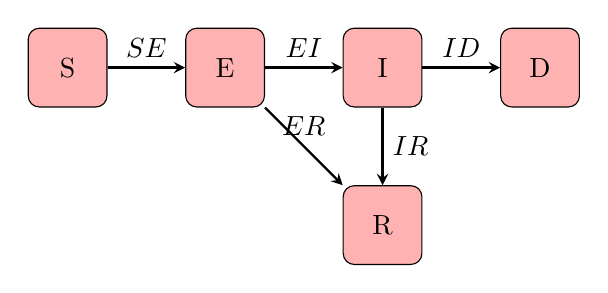
\begin{tikzpicture}[node distance=2cm]
        \node[startstop](S){S};
        \node[startstop,right of=S](E){E};
        \node[startstop,right of=E](I){I};
        \node[startstop,right of=I](D){D};
        \node[startstop,below of=I](R){R};
        \draw[arrow](S)--node[above]{$\T{S}{E}$}(E);
        \draw[arrow](E)--node[above]{$\T{E}{I}$}(I);
        \draw[arrow](E)--node[above]{$\T{E}{R}$}(R);
        \draw[arrow](I)--node[right]{$\T{I}{R}$}(R);
        \draw[arrow](I)--node[above]{$\T{I}{D}$}(D);
    \end{tikzpicture}
    \caption{$SEIRD$模型流程图}
\end{figure}
\par 感染者会转变为治愈者或病逝者,
治愈人数和死亡人数均与感染者人数成正比。
\paragraph{详细积分式}
\SEIRD
\subsubsection{$SEIRS$模型}
\par 考虑到治愈者有复发的可能,
康复者有一定比例重新转变为感染者,
在$SEIRD$模型中加入新的传播机制$\T{R}{I}$,
即为$SEIRS$模型。
\paragraph{感染机制}
\begin{align}
    \TP{S}{E}{S(I+E)} \\
    \TP{E}{R}{E}      \\
    \TP{E}{I}{E}      \\
    \TP{I}{R}{I}      \\
    \TP{I}{D}{I}      \\
    \TP{R}{I}{R}
\end{align}
\par 流程图为:
\begin{figure}[H]
    \centering
    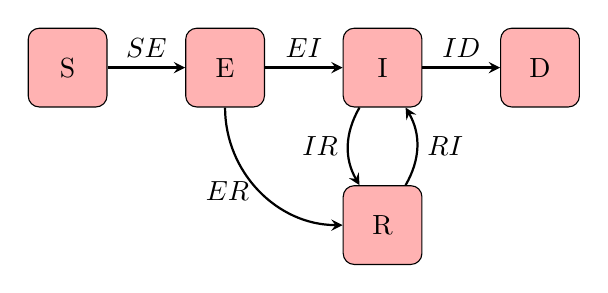
\begin{tikzpicture}[node distance=2cm]
        \node[startstop](S){S};
        \node[startstop,right of=S](E){E};
        \node[startstop,right of=E](I){I};
        \node[startstop,right of=I](D){D};
        \node[startstop,below of=I](R){R};
        \draw[arrow](S)--node[above]{$\T{S}{E}$}(E);
        \draw[arrow](E)--node[above]{$\T{E}{I}$}(I);
        \draw[arrow,out=-90,in=180](E) to node[left]{$\T{E}{R}$}(R);
        \draw[arrow](I)--node[above]{$\T{I}{D}$}(D);
        \draw[arrow,out=-120,in=120](I) to node[left]{$\T{I}{R}$}(R);
        \draw[arrow,out=60,in=-60](R) to node[right]{$\T{R}{I}$}(I);
    \end{tikzpicture}
    \caption{$SEIRD$模型流程图}
\end{figure}
\par 治愈者有可能变为感染者,
之所以不是携带者是因为治愈者已有抗体,
由携带到感染的几率小于易感者,
故感染病毒后不能简单的归入携带者,
所以将其从携带到感染归为一个过程。
\paragraph{详细积分式}
\SEIRS
\subsection{对隔离的处理}
\par 本文并未尝试引入隔离群体的$SEIHR$模型,
因为在该数据中隔离群体是携带者、感染者的混合群体,
且隔离群体有可能治愈或死亡,
而这其中的比例无法通过现有数据得知,
故不能通过拟合来确定其参数。
\par 对于隔离的处理,
本文将数据分为隔离前与隔离后两部分,
对这两个时间段的数据分别进行拟合,
以此来对比隔离前后对疫情传播的影响。
\section{模型拟合}
\subsection{数据源}
\par 拟合所用数据为2020年1月20日至5月1日官方发布的全国疫情数据。
以下为官方发布的疫情数据:
\begin{figure}[H]
    \centering
    \includegraphics[width=\imagewidth]{疫情数据.png}
    \caption{全国疫情数据\label{figure:全国疫情数据}}
\end{figure}
\begin{figure}[H]
    \centering
    \includegraphics[width=\imagewidth]{每日新增人数.png}
    \caption{每日新增人数\label{figure:每日新增人数}}
\end{figure}
\par
由图\ref{figure:全国疫情数据}及图\ref{figure:每日新增人数}可见,
2月12日确诊人数猛增,
是因为当日重新规定了确诊条件,
导致许多疑似病例纳入确诊人数。
\subsection{拟合方法}
\par 本文采取$L-BFGS-B$方法对每个模型进行拟合,
将每个模型的模拟值与真实数据进行对比,
并给出拟合后的参数以及损失值$LOSS$和拟合度$FIT$,
损失值代表了模型拟合的优劣程度,
拟合度代表了模型预测的忧劣程度,
损失值和拟合度将作为本文评判模型优劣的指标。
\par 本文采用前$70\%$的数据进行训练并计算$LOSS$值,
后$30\%$的数据进行验证并计算$FIT$值。
\par 损失值及拟合度定义:
\begin{equation}
    LOSS= FIT = \frac{\sum\limits^{day}\sum\limits^{group}
        (True-Predict)^2}{day}
    \label{math:LOSS}
\end{equation}
\par 式(\ref{math:LOSS})中,
$True$为真实数据,
$Predict$为预测数据,
$LOSS$和$FIT$为计算预测值与真实值的方差后取均值的结果。
\subsection{SIR模型拟合结果}
\showtable{SIR}
\par 因拟合数据较长,将其放在附录\ref{append:数据表},
故在此以图像的形式展示模型拟合结果。
带有“预测”字样的为拟合数据曲线,
不带“预测”字样的为真实数据曲线,
例如在图\ref{figure:SIR模型拟合图像}中,
“预测确诊”和“预测治愈”为模型拟合数据,
“确诊”和“治愈”为真实数据。
\showfigure{SIR}
\par $SIR$模型(表\ref{table:SIR模型拟合参数}、图\ref{figure:SIR模型拟合图像})中$\P{S}{I}$为感染人数增长率,
不同于感染率。
$\P{I}{R}$为治愈人数增长率,
不同于治愈率。
\subsection{SEIR模型拟合结果}
\showtable{SEIR}
\showfigure{SEIR}
\par $SEIR$模型(表\ref{table:SEIR模型拟合参数}、图\ref{figure:SEIR模型拟合图像})中$\P{E}{R}$极低,
一可理解为潜伏期较长,
二可理解为致病率较高,
这两点都与实际情况吻合。
\subsection{SEIRD模型拟合结果}
\showtable{SEIRD}
\showfigure{SEIRD}
\par $SEIRD$模型(表\ref{table:SEIRD模型拟合参数}、图\ref{figure:SEIRD模型拟合图像})中$\P{I}{D}$为预测死亡增长率,
不同于死亡率。
\subsection{SEIRS模型拟合结果}
\showtable{SEIRS}
\showfigure{SEIRS}
\par $SEIRS$模型(表\ref{table:SEIRS模型拟合参数}、图\ref{figure:SEIRS模型拟合图像})中的$\P{R}{I}=0.001$,
可以理解为复阳率极低,
说明复阳人数占患病人数比例极低,
对疫情的影响微乎其微。
\subsection{考虑隔离的模型拟合结果}
\par 对比各个模型拟合前后的参数值变化:
\showtables{SIR}
\showfigures{SIR}
\par 在$SIR$模型(表\ref{table:SIR模型隔离前后拟合参数}、图\ref{figure:SIR模型隔离前后拟合图像})中,
$\P{S}{I}$有所下降,
$\P{I}{R}$有所增减,
代表感染率降低,
治愈率提高。
\showtables{SEIR}
\showfigures{SEIR}
\par 在$SEIR$模型(表\ref{table:SEIR模型隔离前后拟合参数}、图\ref{figure:SEIR模型隔离前后拟合图像})中,
$\P{S}{E},\P{E}{I}$有所下降,
$\P{I}{R}$有所增减,
代表感染率降低,
治愈率提高。
\showtables{SEIRD}
\showfigures{SEIRD}
\par 在$SEIRD$模型(表\ref{table:SEIRD模型隔离前后拟合参数}、图\ref{figure:SEIRD模型隔离前后拟合图像})中,
$\P{S}{E}$、
$\P{E}{I}$有所下降,
$\P{S}{E}\cdot \P{E}{I}$有所下降,
$\P{I}{R}$有所增加,
$\P{I}{D}$有所下降
代表患病率降低,
治愈率提高,
死亡率降低。
\showtables{SEIRS}
\showfigures{SEIRS}
\par $SEIRS$模型(表\ref{table:SEIRS模型隔离前后拟合参数}、图\ref{figure:SEIRS模型隔离前后拟合图像})
与$SEIRD$模型(表\ref{table:SEIRD模型隔离前后拟合参数}、图\ref{figure:SEIRD模型隔离前后拟合图像})
的参数十分接近,
无论分段与否,$SEIRS$模型的$\P{S}{I}$均为$0.001$,
说明$\P{S}{I}$对模型的影响极其微弱。
\subsection{结果分析}
\par 仅从$LOSS$值判断,
模型从优到劣排序为$SEIRD>SEIRS>SEIR>SIR$。
\par 仅从$FIT$值判断,
模型从优到劣排序为$SEIRD>SIR>SEIR>SEIRS$。
\par 综合考虑$LOSS$值及$FIT$值的大小,
认为在上述几种模型中,
$SEIRD$模型最适用于该类传染病预测。
\par 无论哪种模型,
比较模型分段前后参数,
均可得出传染病的传染率降低、治愈率增加、死亡率降低这一结论。
\par 本文使用基础再生数$R_0$和有效再生数$R_t$两个参数来评估疫情传播情况:
\par 基础再生数$R_0$为自然状态下,
平均一个患者可以传染的人数。
$R_0$常用来描述疫情传播速率,
可以通过$R_0$来反映一个传染病的爆发力和严重程度。
\par 有效再生数$R_t$是指加上防控手段后,
平均一个患者可以传染的人数,
$R_t$的计算公式与$R_0$相同。
\par $R_0$($R_t$)的计算公式为\cite{应用SEIR模型预测2009年甲型H1N1流感流行趋势,王宝童2013流感传播数学模型的基本再生数}:
\begin{equation}
    R_0(R_t) = \frac{\P{S}{I}}{\P{I}{R}}
    = \frac{\P{S}{E}\cdot \P{E}{I}}{\P{I}{R}}
    \label{math:R0计算公式}
\end{equation}
\par 根据表\ref{table:SEIRD模型拟合参数}依据式(\ref{math:R0计算公式})
可计算出总体的有效生殖数$R_t=1.754$,
与官方发布数据$1.4\sim 3.8$相符。
\par 根据表\ref{table:SEIRD模型隔离前后拟合参数}计算出隔离前基本生殖数$R_0=5.937$及隔离后有效生殖数$R_t=1.081$,
可见在防控措施下疫情传播得到了有效遏制。
其中计算所得$R_0$符合疫情早期爆发情况下的基本生殖数估计值$4.16\leq R_0\leq 7.10$\cite{协调基本生殖数量及其不确定性的早期暴发估计:新型冠状病毒(SARS-CoV-2)暴发的框架和应用},
略高于2020年2月8日前的基本生殖数估计值$3.63\leq R_0\leq 5.13$\cite{估计2019年新型冠状病毒的流行性:数学建模研究},
考虑到本文以2020年2月12日为分界线,
此时正处于疫情爆发时间,
所得结论可以接受。

\section{结论}
\subsection{总结}
\subsection{创新点}
\begin{itemize}
    \item 对数据进行分段拟合
\end{itemize}
\subsection{不足及展望}
\begin{itemize}
    \item 模型所采用参数为固定值,
          实际情况中应为随时间动态变化的序列,
          但所采用的拟合方式只能用于优化参数为固定值的模型。
\end{itemize}
% 目录生成参考文献
\clearpage
\normalsize
\bibliography{paper.bib}
\addcontentsline{toc}{section}{参考文献}
\clearpage
\vspace{2cm}
\begin{center}
      \textbf{\zihao{1}\heizi致谢}
\end{center}
\vspace{2cm}
\par 本文
\par 十分感谢指导教师王斌,
从选题到为本文提出了许多宝贵的意见。
\addcontentsline{toc}{section}{致谢}
\clearpage
% \zihao{-4}
% \begin{appendix}
    \section{数据\label{appendix:数据}}
    以下为官方发布的疫情数据:
    \\
    \includegraphics[width=\imagewidth]{疫情数据.png}
    \\
    \includegraphics[width=\imagewidth]{每日新增人数.png}
    \par
    2月12日确诊人数猛增,
    是因为当日重新规定了确诊条件,
    导致许多疑似病例纳入确诊人数。
    \section{模型积分式\label{appendix:模型积分式}}
    \begin{table}[H]
        \centering
        \caption{人群}
        \begin{tabular}{ll}
            \hline
            符号 & 含义   \\
            \hline
            $S$  & 易感者 \\
            $I$  & 感染者 \\
            $R$  & 康复者 \\
            $E$  & 携带者 \\
            $D$  & 病逝者 \\
            \hline
        \end{tabular}
    \end{table}
    \subsection{SIR}
    \begin{table}[H]
        \centering
        \caption{SIR模型参数表}
        \begin{tabular}{ll}
            \hline
            符号     & 含义         \\
            \hline
            $\alpha$ & \PText{S}{I} \\
            $\beta$  & \PText{I}{R} \\
            \hline
        \end{tabular}
    \end{table}
    \def\SI{IS\alpha}
    \def\IR{I\beta}
    \begin{align}
        \dt{S} & = -\SI      \\
        \dt{I} & = \SI - \IR \\
        \dt{R} & = \IR
    \end{align}
    \subsection{SEIR}
    \begin{table}[H]
        \centering
        \caption{SEIR模型参数表}
        \begin{tabular}{ll}
            \hline
            符号     & 含义         \\
            \hline
            $\alpha$ & \PText{S}{E} \\
            $\gamma$ & \PText{E}{I} \\
            $\beta$  & \PText{I}{R} \\
            \hline
        \end{tabular}
    \end{table}
    \def\SE{(I+E)S\alpha}
    \def\EI{E\gamma}
    \def\IR{I\beta}
    \begin{align}
        \dt{S} & = -\SE      \\
        \dt{E} & = \SE - \EI \\
        \dt{I} & = \EI - \IR \\
        \dt{R} & = \IR
    \end{align}
    \subsection{SEIRD}
    \begin{table}[H]
        \centering
        \caption{SEIRD模型参数表}
        \begin{tabular}{ll}
            \hline
            符号     & 含义         \\
            \hline
            $\alpha$ & \PText{S}{E} \\
            $\gamma$ & \PText{E}{I} \\
            $\beta$  & \PText{I}{R} \\
            $\delta$ & \PText{I}{D} \\
            \hline
        \end{tabular}
    \end{table}
    \def\SE{(I+E)S\alpha}
    \def\EI{E\gamma}
    \def\IR{I\beta}
    \def\ID{I\delta}
    \begin{align}
        \dt{S} & = -\SE            \\
        \dt{E} & = \SE - \EI       \\
        \dt{I} & = \EI - \IR - \ID \\
        \dt{R} & = \IR             \\
        \dt{D} & = \ID
    \end{align}
    \subsection{SEIRS}
    \begin{table}[H]
        \centering
        \caption{SEIRS模型参数表}
        \begin{tabular}{ll}
            \hline
            符号     & 含义         \\
            \hline
            $\alpha$ & \PText{S}{E} \\
            $\gamma$ & \PText{E}{I} \\
            $\beta$  & \PText{I}{R} \\
            $\delta$ & \PText{I}{D} \\
            $\theta$ & \PText{R}{I} \\
            \hline
        \end{tabular}
    \end{table}
    \def\SE{(I+E)S\alpha}
    \def\EI{E\gamma}
    \def\IR{I\beta}
    \def\ID{I\delta}
    \def\RI{R\theta}
    \begin{align}
        \dt{S} & = -\SE                  \\
        \dt{E} & = \SE - \EI             \\
        \dt{I} & = \RI + \EI - \IR - \ID \\
        \dt{R} & = \IR - \RI             \\
        \dt{D} & = \ID                   \\
    \end{align}
    \section{数据拟合结果\label{appendix:数据拟合结果}}
    \subsection{SIR}
    \showfigure{SIR}
    \showfigures{SIR}
    \subsection{SEIR}
    \showfigure{SEIR}
    \showfigures{SEIR}
    \subsection{SEIRD}
    \showfigure{SEIRD}
    \showfigures{SEIRD}
    \subsection{SEIRS}
    \showfigure{SEIRS}
    \showfigures{SEIRS}
\end{appendix}
\end{document}